\documentclass[11pt]{article}
\usepackage{graphicx}
\usepackage[margin=1.5in,left=1.4in, includefoot]{geometry}

\begin{document}
\begin{titlepage}

\textbf{Bangabandhu Sheikh Mujibur Rahman Science and Technology}
\begin{center}
\textbf{University\\}

\bigskip
\bigskip
\bigskip
\medskip
\bigskip
\bigskip
\medskip

Technical writing and presentation\\
\line(1,0){150}\\
[5mm]
\huge {\bfseries Report\\}

\line(1,0){100}\\
[.5mm]
\textsc{\Large Dynamic Programming}

\end{center} 
\vfill

\begin{flushright}

\textbf{\large Sayad Bin Kamrul\\}
Dept. of CSE\\ 
ID: 18ICTCSE036\\

\end{flushright}
\end{titlepage}

\section*{Introduction of Dynamic Programming\\}
Dynamic Programming is the most powerful design technique for solving optimization problems.\\
Divide and Conquer algorithm partition the problem into disjoint subproblems solve the subproblems recursively and then combine their solution to solve the original problems.\\
Dynamic Programming is used when the subproblems are not independent, e.g. when they share the same subproblems. In this case, divide and conquer may do more work than necessary, because it solves the same sub problem multiple times.\\
Dynamic Programming solves each subproblems just once and stores the result in a table so that it can be repeatedly retrieved if needed again.\\
Dynamic Programming is a Bottom-up approach- we solve all possible small problems and then combine to obtain solutions for bigger problems.\\
Dynamic Programming is a paradigm of algorithm design in which an optimization problem is solved by a combination of achieving sub-problem solutions and appearing to the "principle of optimality".\\

\section*{Characteristics of Dynamic Programming}

Dynamic Programming works when a problem has the following features:\\
\subsection*{Optimal Substructure:} If an optimal solution contains optimal sub solutions then a problem exhibits optimal substructure.

\subsection*{Overlapping subproblems:} When a recursive algorithm would visit the same subproblems repeatedly, then a problem has overlapping subproblems.\\

\paragraph*{} If a problem has optimal substructure, then we can recursively define an optimal solution. If a problem has overlapping subproblems, then we can improve on a recursive implementation by computing each subproblem only once.
\paragraph*{}If a problem doesn't have optimal substructure, there is no basis for defining a recursive algorithm to find the optimal solutions. If a problem doesn't have overlapping sub problems, we don't have anything to gain by using dynamic programming.
\begin{figure}
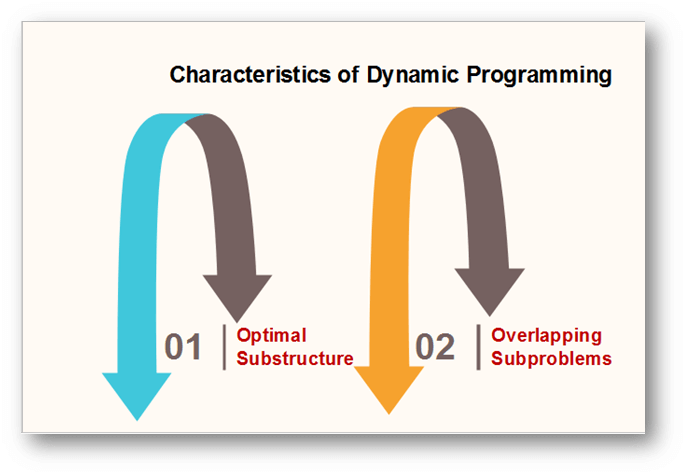
\includegraphics[width=.8\textwidth]{1.png}
\end{figure}
\paragraph*{}If the space of subproblems is enough (i.e. polynomial in the size of the input), dynamic programming can be much more efficient than recursion.
\section*{Elements of Dynamic Programming}

There are basically three elements that characterize a dynamic programming algorithm:-
\begin{figure}
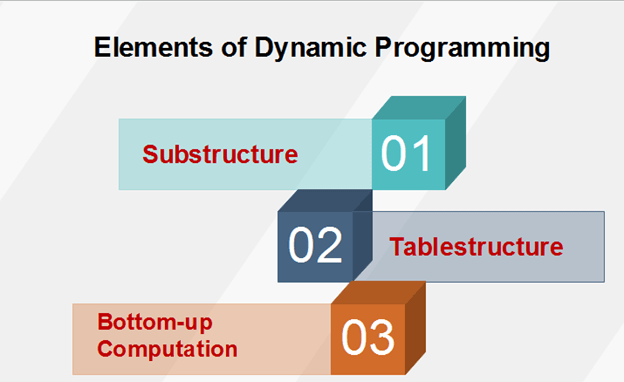
\includegraphics[width=.8\textwidth]{2.png}
\end{figure}
\subsection*{1. Substructure:}
Decompose the given problem into smaller subproblems. Express the solution of the original problem in terms of the solution for smaller problems.\\
\subsection*{2. Table Structure:}
Table Structure: After solving the sub-problems, store the results to the sub problems in a table. This is done because subproblem solutions are reused many times, and we do not want to repeatedly solve the same problem over and over again.\\
\subsection*{3. Bottom-up Computation:}
Bottom-up Computation: Using table, combine the solution of smaller subproblems to solve larger subproblems and eventually arrives at a solution to complete problem.\\

\section*{Components of Dynamic programming\\}
\begin{figure}
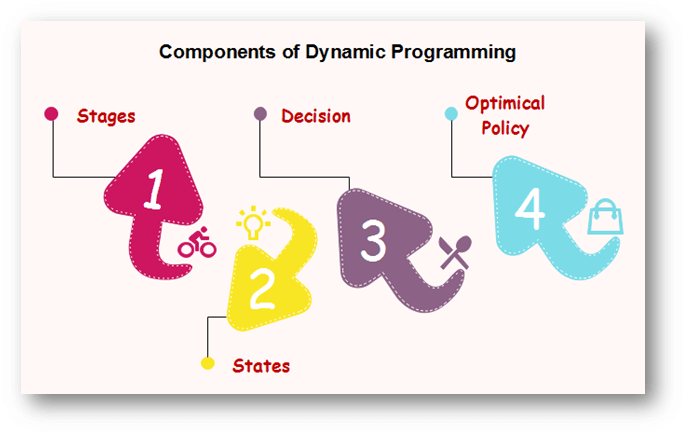
\includegraphics[width=.8\textwidth]{3.png}
\end{figure}
\subsection*{1. Stages:}
The problem can be divided into several subproblems, which are called stages. A stage is a small portion of a given problem. For example, in the shortest path problem, they were defined by the structure of the graph.\\
\subsection*{2. States:}
Each stage has several states associated with it. The states for the shortest path problem was the node reached.\\
\subsection*{3. Optimal policy:}
It is a rule which determines the decision at each stage; a policy is called an optimal policy if it is globally optimal. This is known as Bellman principle of optimality.\\\\
\textbf{5.} Given the current state, the optimal choices for each of the remaining states does not depend on the previous states or decisions. In the shortest path problem, it was not necessary to know how we got a node only that we did.\\\\
\textbf{6.} There exist a recursive relationship that identify the optimal decisions for stage j, given that stage j+1, has already been solved.\\\\
\textbf{7.} The final stage must be solved by itself.\\

\section*{Development of Dynamic Programming Algorithm}
It can be broken into four steps:\\\\
\textbf{1.} Characterize the structure of an optimal solution.\\\\
\textbf{2.} Recursively defined the value of the optimal solution. Like Divide and Conquer, divide the problem into two or more optimal parts recursively. This helps to determine what the solution will look like.\\\\
\textbf{3.} Compute the value of the optimal solution from the bottom up (starting with the smallest subproblems)\\\\
\textbf{4.} Construct the optimal solution for the entire problem form the computed values of smaller subproblems.\\ 

\section*{Applications of dynamic programming\\}

\textbf{1.} 0/1 knapsack problem.\\\\
\textbf{2.} Mathematical optimization problem.\\\\
\textbf{3.} All pair Shortest path problem.\\\\
\textbf{4.} Reliability design problem.\\\\
\textbf{5.} Longest common subsequence (LCS)\\\\
\textbf{6.} Flight control and robotics control.\\\\
\textbf{7.} Time-sharing: It schedules the job to maximize CPU usage.\\\\


\end{document}';lkj